\documentclass{article}

\usepackage{times}
\usepackage{uist}

%\usepackage{mathptmx}
\usepackage{graphicx}
%\usepackage{subfig}
%\usepackage{url}
%\usepackage{wrapfig}

\begin{document}

% --- Copyright notice ---
\conferenceinfo{UIST'12}{October 7-10, 2012, Cambridge, MA, USA}
\CopyrightYear{2012}
\crdata{978-1-xxxx-xxxx-x}

% Uncomment the following line to hide the copyright notice
% \toappear{}
% ------------------------

\bibliographystyle{plain}

\title{Poster: A link between physical and digital drawing \\
       through spatial augmented reality}

%%
%% Note on formatting authors at different institutions, as shown below:
%% Change width arg (currently 7cm) to parbox commands as needed to
%% accommodate widest lines, taking care not to overflow the 17.8cm line width.
%% Add or delete parboxes for additional authors at different institutions. 
%% If additional authors won't fit in one row, you can add a "\\"  at the
%% end of a parbox's closing "}" to have the next parbox start a new row.
%% Be sure NOT to put any blank lines between parbox commands!
%%

\author{
\parbox[t]{9cm}{\centering
	     {\em Jeremy Laviole}\\
	     Univ. Bordeaux, LaBRI, UMR 5800, F-33400 Talence, France.\\
         CNRS, LaBRI, UMR 5800, F-33400 Talence, France.\\
	     Inria, F-33400 Talence, France.\\
	     laviole@labri.fr}
\parbox[t]{9cm}{\centering
	     {\em Martin Hachet}\\
	     Inria, F-33400 Talence, France.\\
	     LaBRI, UMR 5800, F-33400 Talence, France.\\
	     martin.hachet@inria.fr}
}

\maketitle

\abstract

Physical drawing is being more and more replaced by digital drawing. The digital world offers a wide range and tools and techniques that does not apply in the real world. In the physical world, every error will leave a mark, but it contributes to the uniqueness of the result. In this paper, we propose some basic tools to link physical drawing and digital drawing through spatial augmented reality (SAR). These tools enables a wide variety of new uses of drawing software such as The Gimp~\cite{gimp2004image}. 


\classification{H5.2 [Information interfaces and presentation]:
User Interfaces. - Graphical user interfaces.}

\terms{Design, Human Factors (Your general terms must be any of the
  following 16 designated terms: Algorithms, Management, Measurement,
  Documentation, Performance, Design, Economics, Reliability,
  Experimentation, Security, Human Factors, Standardization,
  Languages, Theory, Legal Aspects, Verification. See ~\cite{ACMTerms} for more details.)}

\keywords{Guides, instructions, formatting.}

\tolerance=400 
  % makes some lines with lots of white space, but 	
  % tends to prevent words from sticking out in the margin

\section{INTRODUCTION}

Software for digital creations are getting richer and allows a wide variety of creation and styles. They allow purely digital tools such as a clone brush or the use of loads of layers. Some of them also try to recreate physical drawing tools and techniques (cite digital wet paint etc...). 

Physical drawing is very different from digital drawing, the creation is unique. The uniqueness is an important feature, it creates a link between the artist and the creation that is harder to achieve with a computer. The drawing or painting can be transported, has to be taken care of, and it will age. The whole creation process requires to buy materials, and each material will provide a different experience. The smell, contact with paper and the experience to master the different tools provide a creative experience very different to the digital one. 

In this paper, we propose to use classical digital creation tools for physical artistic creations. To achieve this, the drawing is captured and sent to the drawing software. Then, the user can add new elements such as continuing shapes or colouring parts and project the additions on the physical drawing.   


\section{System overview}

%\subsection{Spatial augmented reality}

The Spatial augmented reality (SAR) is composed of a projector camera system (procam), an additional high resolution camera to capture the drawings, and a pen and tablet for stylus input. A multi-touch input is also available using a depth camera. For a detailed description of the procam system, please have a look at~\cite{laviole:2012}. It allows fast tracking of paper sheet and projection inside it. The tracking latency is not an issue for this kind of application, but the projection precision is the current limitation. Although high resolution cameras are relatively cheap, high resolution projection can be very expensive, the current projection precision is about 1 pixel/mm. 


\begin{figure}[tb]
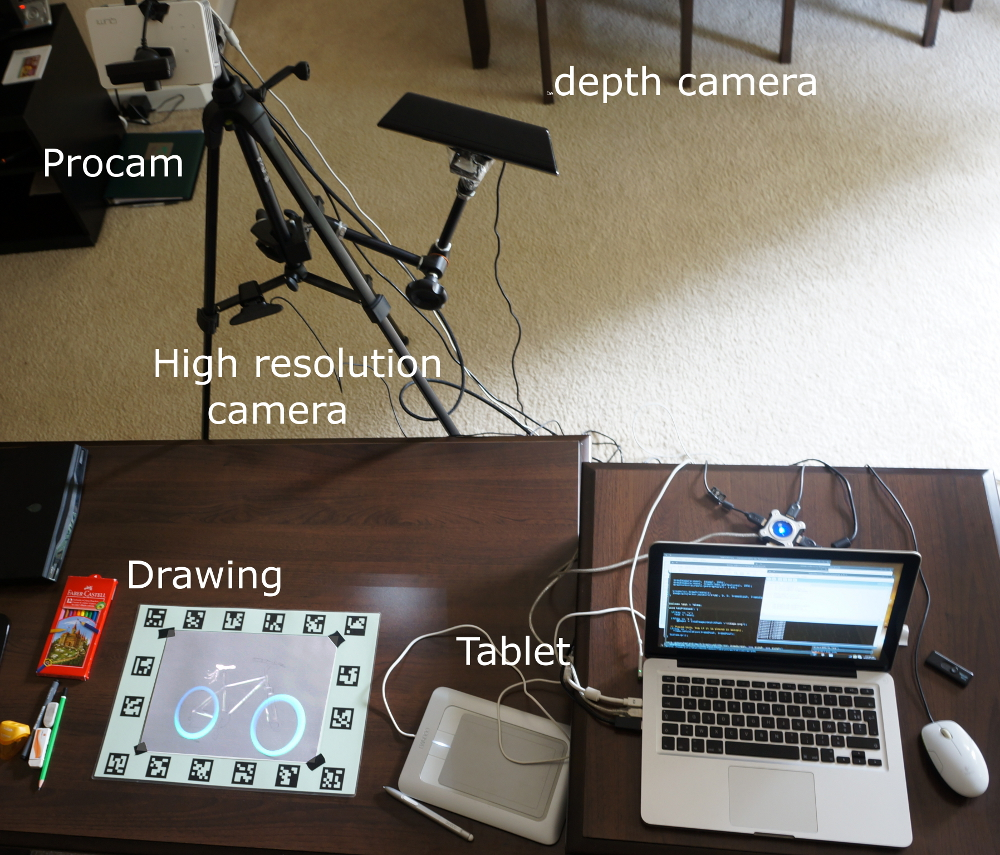
\includegraphics[width = 73mm]{DSC00299-2-rogne-annote.JPG}
\caption{A figure caption.  It is set in 9 point Helvetica type, with a
0.5 cm wider margin on both left and right sides.} 
\label{fig:setup}
\end{figure}

The transfer from the physical world to the digital world is made by a high resolution web camera. Only the drawing is extracted from the image and save to the disk. (ref image ?). The image can be opened with an image edition software. In this paper we chose to use The Gimp, but any edition software can be used. Once the image is imported, a drawing layer has to be created. The edition of the drawing will be made on this layer and the projection will consist only in this layer. Once the  layer is done, the user can save this layer and hit the load button in the SAR tool. Consequently the physical drawing will contain the added digital informations.  

In order to make the system more direct, we also included some digital drawing tools into our SAR software. Some basic elements such as line, curve and freehand drawing can be done directly. The lines and curves have control points which can be placed directly using the touch interface. The tablet device allows the user to draw digital lines onto the real drawing. In the next section, we describe how to use our system by a demonstration on a simple example. 




%% TODO: figure : drawing, capture, reprojection...  
\begin{figure}[t]
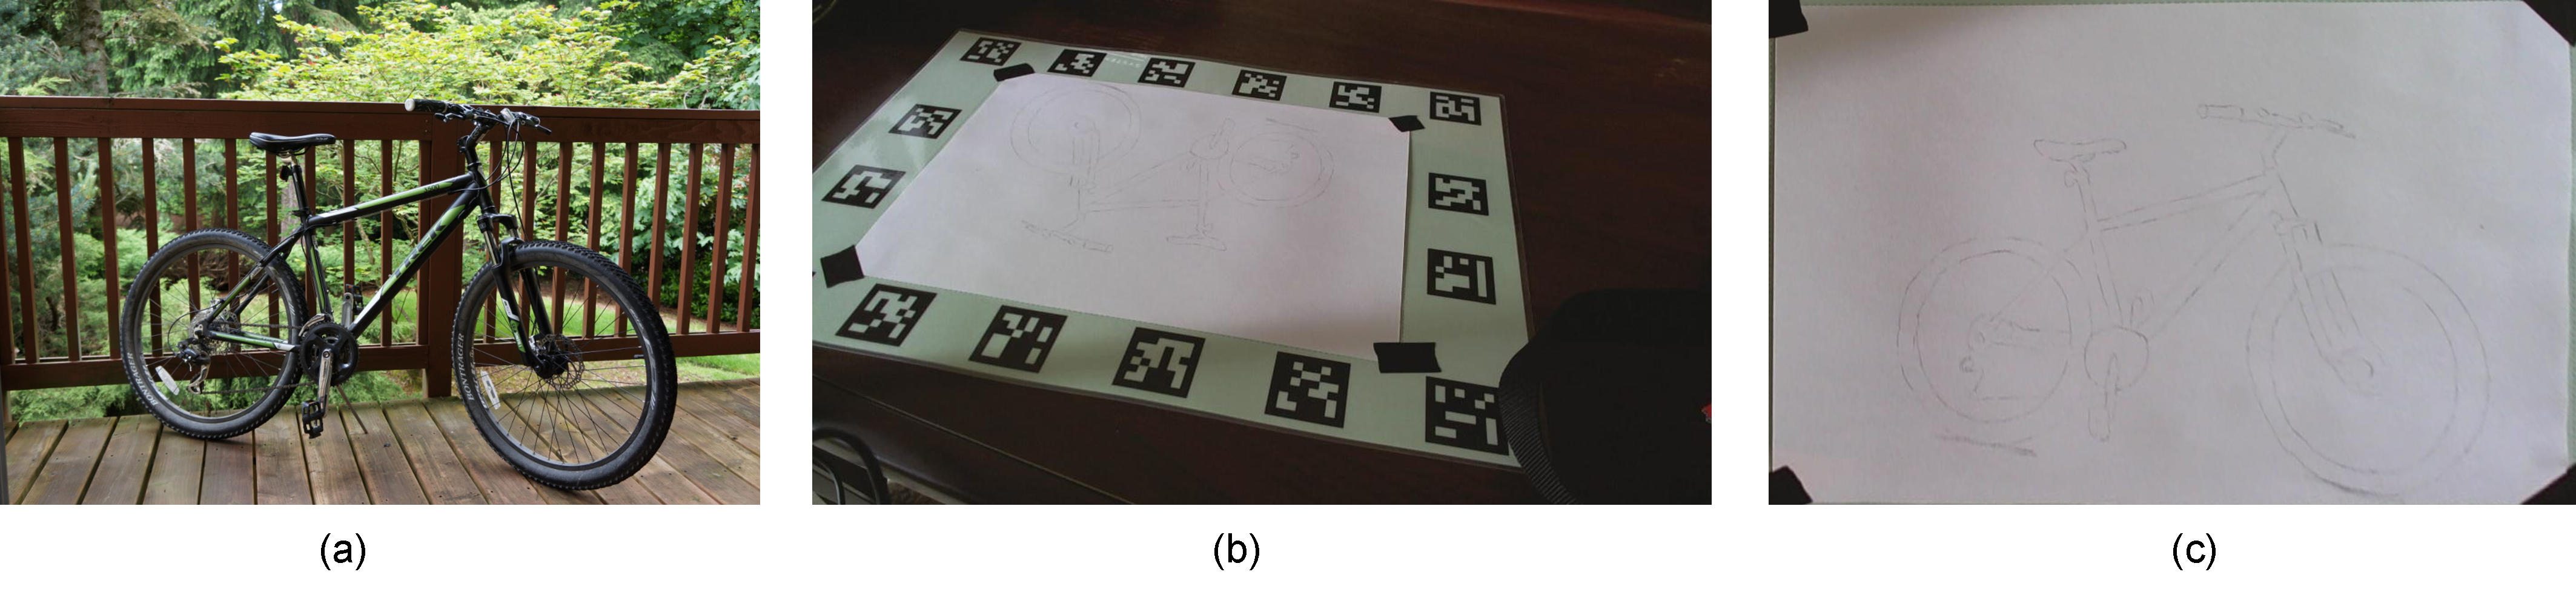
\includegraphics[width = 85mm]{fig1.pdf}
\caption{A figure caption.  It is set in 9 point Helvetica type, with a
0.5 cm wider margin on both left and right sides.} 
\label{fig:1}
\end{figure}

\section{Example use}

In this example, we show the firsts steps of the creation of a drawing using our system. We start by a photo (fig ...) projected on a paper sheet. The artist uses the projection to draw the first contours of the bike. Once it is done, the drawing is captured by a camera (fig ...) and the drawing is extracted (fig ...). It is then exported to the drawing software and added as a layer on the first image, as illustrated in Figure. 
In the drawing software, we decided to try different looks for the bike by selecting the texture elements from the bike and adding coloured wheels. In the image edition software, the user can have a preview of the projection, by mixing the captured image and the new layer (fig.). Then, only the layer is projected  (fig ..). From this, the user can continue the physical drawing, or add digital elements using the tablet and digital construction line tools (fig...). The physical drawing and digital elements can be captured and saved, then imported into the edition software and so on. 

\begin{figure}[b]
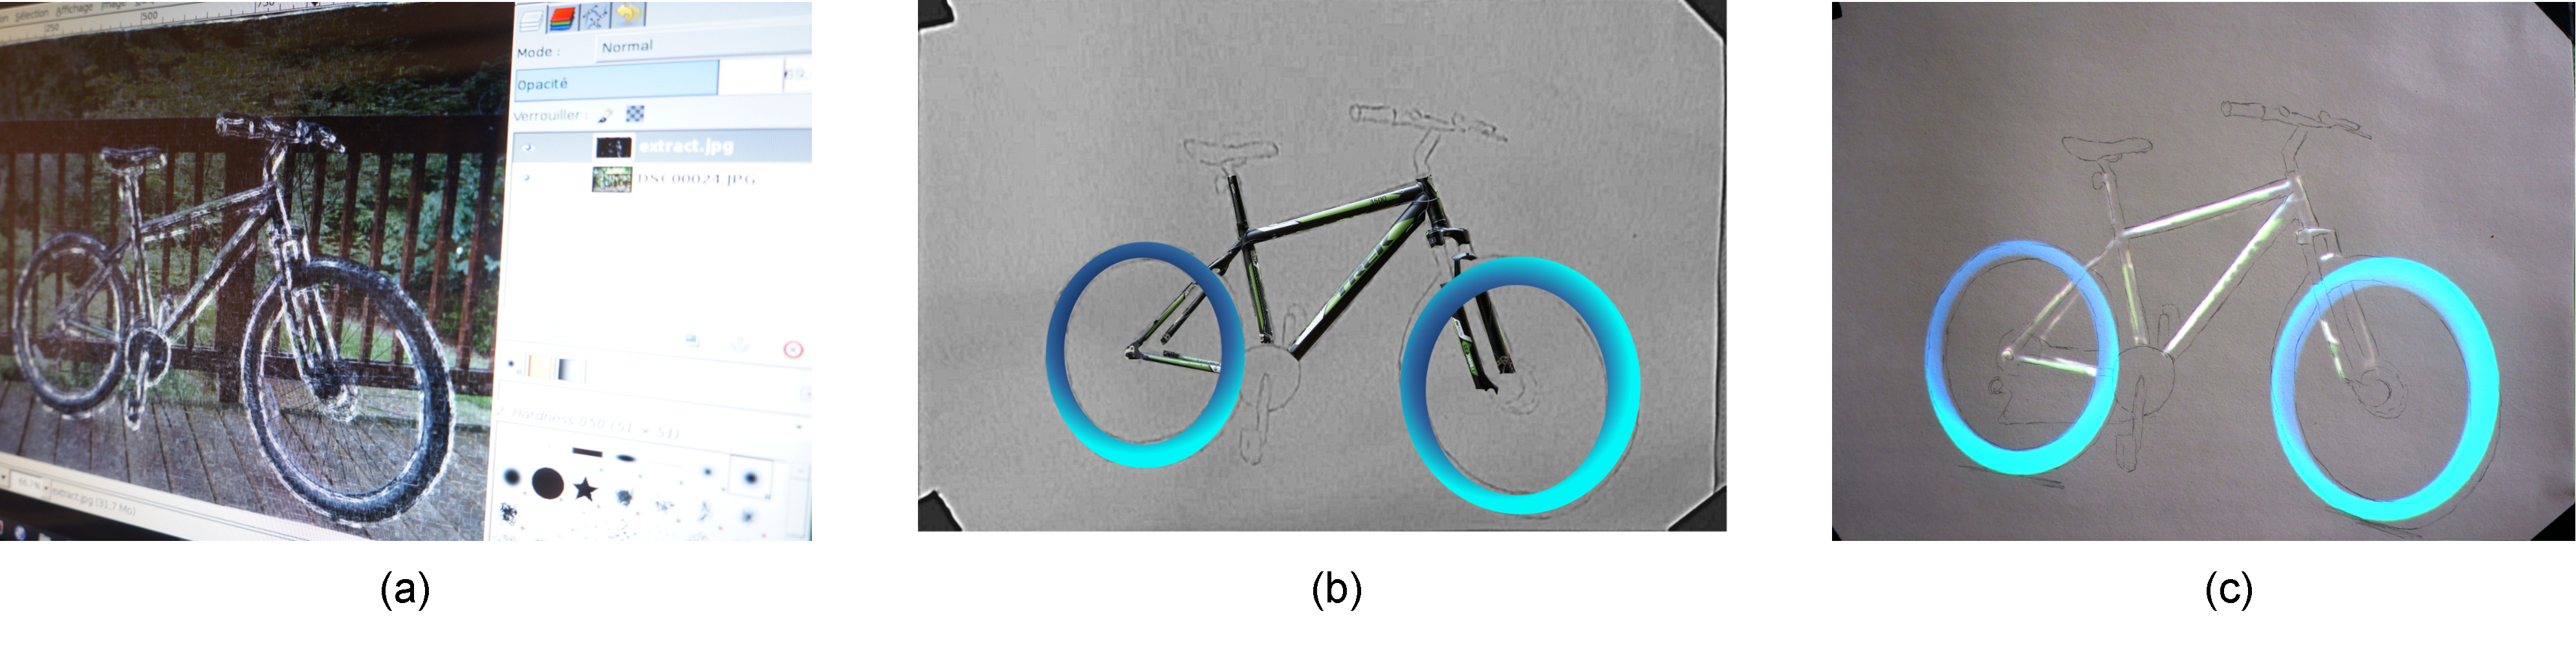
\includegraphics[width = 85mm]{fig2.pdf}
\caption{A figure caption.  It is set in 9 point Helvetica type, with a
0.5 cm wider margin on both left and right sides.} 
\label{fig:2}
\end{figure}

\section{Extensions}

An interesting extension will be to calibrate the color of the physical tools with the projection. Using this, we would be able to simulate real colors, and result from the a specific colored pen or paint. Different pressure, or type of application could be calibrated and imported into the edition software. This way the artist could try appearances with various quantities of paint, or different pressures on a pen. This kind of feature promises future drawings, but the realisation will still be made by the artist; consequently adding some uncertainty and uniqueness on the result. 

The main extension would be to create a drawing software integrating the capture and projection. This kind of software creates interesting design challenges, and will raise the question of the utility of a computer and mouse / keyboard interfaces. Every software tools such as palettes and layer switching could be made using touch tangible menus, such as in (papart). 

\begin{figure}[b]
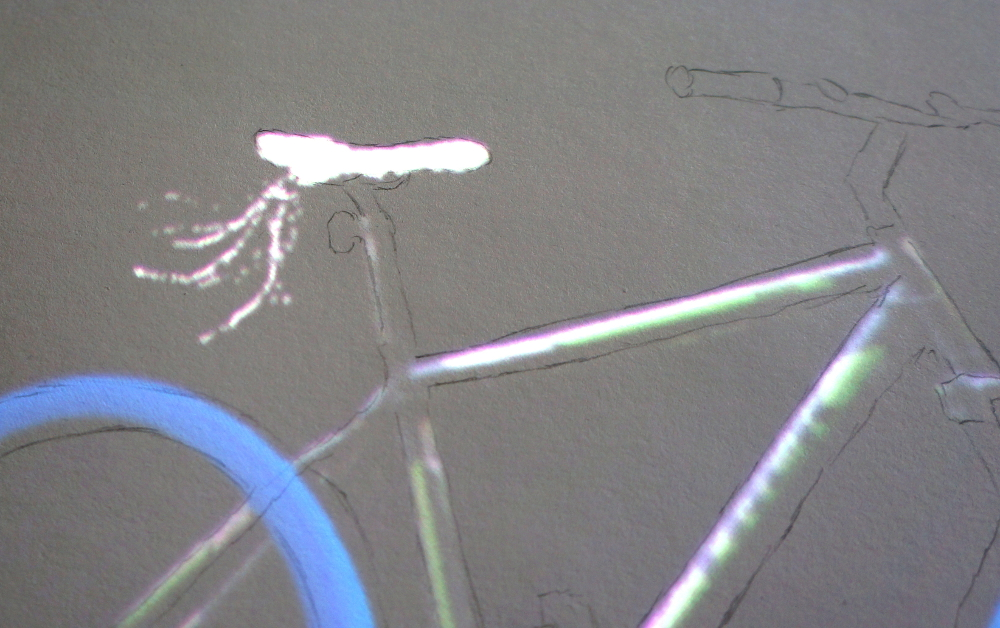
\includegraphics[width = 85mm]{velo4.JPG}
\caption{A figure caption.  It is set in 9 point Helvetica type, with a
0.5 cm wider margin on both left and right sides.} 
\label{fig:zoom}
\end{figure}

\section{Conclusion}

In this paper we proposed SAR tools which merges physical drawing and current drawing software. It allows quick transfer between the physical drawing to the drawing software and vice versa. 
...



\bibliographystyle{abbrv}
\bibliography{paper}


\end{document}
